\documentclass{article}
% the following gives us one-inch margins:
\usepackage[margin=1in]{geometry}
% this allows us to insert .png, .gif, .jpg, etc.:
\usepackage{graphicx}
% this allows us to show verbatim stuff, like code,
% and put fancy boxes around it:
\usepackage{fancyvrb}
% this allows us to insert links to the internet:
\usepackage{hyperref}
% this has a bunch of cool math stuff not part of the standard library:
\usepackage{amsfonts,amssymb,amsmath}
% this is a cool drawing package, and some libraries for automata:
\usepackage{tikz}
\usepackage{xspace}
\newcommand{\TikZ}{Ti\textit{k}Z\xspace}

\usetikzlibrary{arrows,automata}

% new commands for frequently used stuff:
\newcommand{\qed}{\hfill\ensuremath{\blacksquare}}
\newcommand{\R}{\mathbb{R}}
\newcommand{\N}{\mathbb{N}}

\title{Some \LaTeX{} examples}
\author{Geoffrey Matthews}

\begin{document}
\maketitle

\section{Mechanics}
This file contains some examples to get you started using \LaTeX{} to
typeset mathematics.  It is the premiere software for technical
publications.  Good places to get started with tutorials: 
\begin{itemize}
\item \url{http://www.latex-tutorial.com/}
\item \url{http://www.stdout.org/~winston/latex/latexsheet.pdf}
\end{itemize}

To compile a \LaTeX{} file, {\tt myfile.tex} to {\tt myfile.pdf}, 
in the labs, simply enter the
following command in a terminal window:
\begin{Verbatim}[frame=single]
pdflatex myfile.tex
\end{Verbatim}
or use a GUI such as TexWorks or TexStudio.

You can also get your \LaTeX{} processed online at
\url{https://www.overleaf.com/}.

\section{Some example text}
Here is some inline math:  $\sum_{i=1}^{n} i^2$ and
here is the same thing with display math:
\[
\sum_{i=1}^{n} i^2
\]
Here is a set of equations lined up nicely:
\begin{align*}
(a+b)^2 &= (a+b)(a+b) \\
        &= a(a+b) + b(a+b) \\
        &= a^2 + ab + ba + b^2  & \mbox{Here is a comment on a line!}\\
        &= a^2 + 2ab + b^2      & \mbox{Another comment}
\end{align*}

You can talk about the real numbers, $\R$, the integers $\mathbb{Z}$, the
rational numbers $\mathbb{Q}$, and the natural numbers,
$\N$, using nice fonts.  Notice how I made new commands for some of these in
the preamble, to simplify typing.
Here is an enumerated list:
\begin{enumerate}

\item $\mathcal{P}(\{1,2,3\}) \subseteq \mathcal{P}(\{1,2,3,4\})$

\item
$
\bigcup_{i\in\N}i^2 = \{0,1,4,9,\ldots\}
$

\item
\[
\bigcap_{i\in\N}i^2 \not= \{0,1,4,9,\ldots\}
\]

\end{enumerate}

\section{Figures}

You can also include and scale figures.
I drew the picture shown in Figure \ref{setfigure}
with a simple paint program, saved it as a {\tt .png}
file, and imported it into this document.


\begin{figure}
  \begin{center}
    \includegraphics[scale=0.5]{sets.png}
    \caption{A diagram of some sets.}
    \label{setfigure}
  \end{center}
\end{figure}

You can also include figures inline, like this:
\includegraphics[scale=0.25]{sets.png} but it looks weird sometimes.

Later on, we'll see how to make spectacular diagrams using the \TikZ
package. 

\section{Solutions to Some Exercises From the Book of Proof}


{\bf Note:  These problems are all solved in the book.  I include their
solutions here to demonstrate how to typeset them in \LaTeX.}

\begin{description}

\item[Chapter 1 Exercises]
\item[Section 1.1]
\item[1.] $\{5x-1:x\in\mathbb{Z}\} = \{...,-11,-6,-1,4,9,14,19,24,29,...\}$
\item[13.] $\{x\in\mathbb{Z}:|6x|<5\} = \{0\}$

\item[Section 1.2]
\item[1.]
  \begin{description}
  \item[(a)] $A\times B = \{(1,a),(1,c),(2,a)(2,c),(3,a),(3,c),(4,a),(4,c)\}$
  \end{description}

\item[Section 1.4]
\item[A.] Find the indicated sets.
\begin{description}
\item[3.] $\mathcal{P}(\{\{a,b\},\{c\}\}) = \{\emptyset, \{\{a,b\}\}, \{\{c\}\}, \{\{a,b\},\{c\}\}\}$
\end{description}

\item[B.] Suppose that $|A|=m$ and $|B|=n$. Find the indicated cardinalities.
\begin{description}
\item[13.] $|\mathcal{P}(\mathcal{P}(\mathcal{P}(A)))| = 2^{(2^{(2^m)})}$
\item[15.] $|\mathcal{P}(A\times B)| = 2^{mn}$
\end{description}

\item[Section 1.5]
\item[3.] Suppose $A=\{0,1\}$ and $B=\{1,2\}$.  Find:
\begin{description}
\item[(a)] $A\cup B = \{1,3,4,5,6,7,8,9\}$
\item[(b)] $A\cap B = \{4,6\}$
\end{description}


\item[Section 1.6]
\item[1.] Suppose $A=\{4,3,6,7,1,9\}$ and $B=\{5,6,8,4\}$ have the
  universal set $U=\{n\in\mathbb{Z}:0\leq n \leq 10\}$
  \begin{description}
  \item $\overline{\overline{A} \cap B} = \{0,1,2,3,4,6,7,9,10\}$
  \end{description}

\item[Section 1.8]
\item[5(a)] $\bigcup_{i\in\mathbb{N}} [i,i+1] = [1,\infty)$ or:
  \[\bigcup_{i\in\mathbb{N}} [i,i+1] = [1,\infty)\]

  \item[5(b)] $\bigcap_{i\in\mathbb{N}} [i,i+1] = \emptyset$ or:
    \[\bigcap_{i\in\mathbb{N}} [i,i+1] = \emptyset\]


\item[Chapter 2 Exercises]

\item[Section 2.2]  Express each statement as one of the forms $P\wedge Q$,
  $P\vee Q$, or $\sim P$.  (I will also accept $\neg P$.)
\item [9.] $x\in A-B$

  $(x\in A) \wedge \neg(x\in B)$

\item[Section 2.5]

\item[5.] Write a truth table for $(P\wedge \neg P)\vee Q$
  
  \begin{tabular}{|c|c||c||c|}\hline
    $P$  &   $Q$  & $(P\wedge \neg P)$  &   $(P\wedge \neg P)\vee Q$ \\\hline\hline
    $T$  & $T$  &  $F$  &  {\bf T} \\\hline
    $T$  & $F$  &  $F$  &  {\bf F} \\\hline
    $F$  & $T$  &  $F$  &  {\bf T} \\\hline
    $F$  & $F$  &  $F$  &  {\bf F} \\\hline
  \end{tabular}
  
\item[Chapter 3 Exercises]
\item[Section 3.3]
\item[1.] Suppose a set $A$ has 37 elements.  How may subsets of $A$
  have 10 elements?  How many subsets have 30 elements?  How many have
  0 elements?

  Answers:  ${37 \choose 10} = 348,330,136$ ; ${37 \choose 30} =
  10,295,472$; $ {37 \choose 0} = 1$.

\item[Chapter 4 Exercises]
\item[7.]  Suppose $a,b\in\mathbb{Z}$.  If $a \mid b$, then $a^2 \mid
    b^2$.

    {\em Proof.}  Suppose $a \mid b$.

    By definition of divisibility, this means $b=ac$ for some integer
    $c$.

    Squaring both sides of this equation produces $b^2=a^2c^2$.

    Then $b^2=a^2d$, where $d=c^2\in\mathbb{Z}$.

    By definition of divisibility, this means $a^2 \mid b^2$.
    \qed

\item[Chapter 5 Exercises]

\item[9. Proposition]  Suppose $n\in\mathbb{Z}$.  If $3 \nmid n^2$,
  then $3 \nmid n$.

  {\em Proof.}  (Contrapositive) Suppose it is not the case that
  $3\nmid n$, so $3 \mid n$.  This means that $n=3a$ for some integer
  $a$.  Consequently $n^2 = 9a^2$, from which we get $n^2=3(3a^2)$.
  This shows that there is an integer $b=3a^2$ for which $n^2=3b$,
  which means $3\mid n^2$.  Therefore it is not the case that $3\nmid
  n^2$.  
  \qed

%  \newcommand{\mod}[1]{\ (\mbox{mod}\ #1)}
  
 \item[21. Proposition]  Let $a,b\in\mathbb{Z}$ and $n\in\mathbb{N}$.
   If $a\equiv b \mod{n}$, then $a^3\equiv b^3\mod{n}$.

   {\em Proof.}  (Direct) Suppose $a\equiv b\mod{n}$.  This means
   $n\mid(a-b)$, so there is an integer $c$ for which $a-b=nc$.  Then:
   \begin{align*}
     a-b &= nc\\
     (a-b)(a^2 + ab+b^2) &= nc(a^2 + ab + b^2)\\
     a^3 + a^2b + ab^2 -ba^2 -ab^2 - b^3 &= nc(a^2+ ab + b^2)\\
     a^3 -b^3  &= nc(a^2+ ab + b^2).
   \end{align*}
   Since $a^2 + ab + b^2\in\mathbb{Z}$, the equation $a^3-b^3=nc(a^2+
   ab + b^2)$ implies $n\mid (a^3-b^3)$, and therefore $a^3\equiv
   b^3\mod{n}$.     \qed

\item[Chapter 9 Exercises]
\item[27.] The equation $x^2=2^x$ has three real solutions.

  {\em Proof.}  By inspection, $x=2$ and $x=4$ are two solutions of
  this equation.  But there is a third solution.  Let $m$ be the real
  number for which $m2^m = \frac{1}{2}$.  Then negative number $x=-2m$
  is a solution, as follows.
  \[
  x^2 = (-2m)^2
      = 4m^2
      = 4\left( \frac{m2^m}{2^m} \right)^2
      = 4\left(\frac{\frac{1}{2}}{2^m}\right)^2
      = \frac{1}{2^{2m}}
      = 2^{-2m}
      = 2^x
      \]

\item[Chapter 10 Exercises]

\item[1.] For every integer $n\in\mathbb{N}$, it follows that
  \[
  1 + 2 + 3 + 4 + \ldots + n  = \frac{n^2 + n}{2}
  \]
  or
  \[
  \sum_{i=1}^{n} i  = \frac{n^2 + n}{2}
  \]
  {\bf In this proof I use the second notation.  The book shows the
  solution in the first notation.}

  {\em Proof.}  we will prove this with mathematical induction.

  (1) Observe that if $n=1$, this statement is $1=\frac{1^2 + 1}{2}$,
  which is obviously true.

  (2) Consider any integer $k \geq 1$.  We must show that $S_k$
  implies $S_{k+1}$.  In other words, we must show that if
  \[
  \sum_{i=1}^{k} i = \frac{k^2+k}{2}
  \]
  is true, then
  \[
  \sum_{i=1}^{k+1} i = \frac{(k+1)^2+(k+1)}{2}
  \]
  is also true.  We use direct proof.

  Suppose $k\geq 1$ and 
  \[
  \sum_{i=1}^{k} i = \frac{k^2+k}{2}
  \]
  We observe that
  \begin{align*}
    \sum_{i=1}^{k+1} i
    &= \sum_{i=1}^{k} i + (k+1) &\text{(isolating the last term in the sum)} \\
    &= \frac{k^2+k}{2} + (k+1) & \text{(by the inductive hypothesis)}\\
    &= \frac{k^2 + k + 2(k+2)}{2} \\
    &= \frac{k^2 + 2k + 1 + k + 1}{2}\\
    &= \frac{(k+1)^2 + (k+1)}{2}
  \end{align*}
  Therefore we have shown that 
  \[
  \sum_{i=1}^{k+1} i = \frac{(k+1)^2+(k+1)}{2}
  \]

\end{description}



\section{Some examples typesetting finite automata in \LaTeX{} and \TikZ}

Put the following in your preamble:
\begin{Verbatim}[frame=single]
\usepackage{tikz}
\usetikzlibrary{arrows,automata}
\end{Verbatim}
\newpage
Example figure from the text:\\
\centerline{\includegraphics[scale=0.6]{textdfa}}
We can do {\em much} better with TiKz
\begin{Verbatim}[frame=single]  
  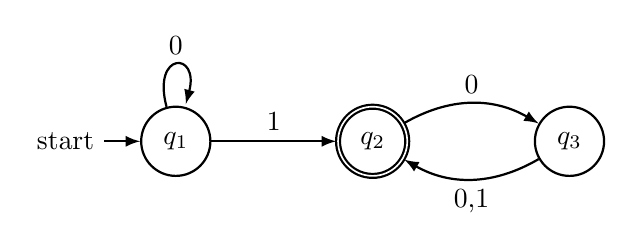
\begin{tikzpicture}[->,>=latex,thick,auto,node distance=2.5cm]
    \node[state,initial] (q1) {$q_1$};
    \node[state,accepting] (q2) [right of=q1] {$q_2$};
    \node[state] (q3) [right of=q2] {$q_3$};
    \path (q1) edge [loop above] node {0} (q1);
    \path (q1) edge node {1} (q2);
    \path (q2) edge [bend left] node {0} (q3);
    \path (q3) edge [bend left] node {0,1} (q2);
  \end{tikzpicture}
\end{Verbatim}
  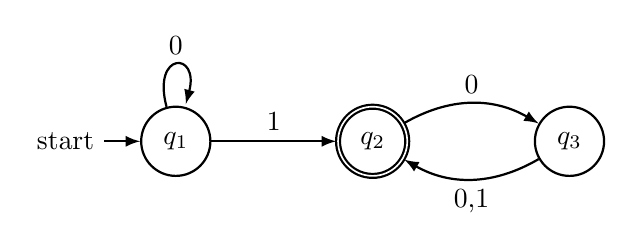
\begin{tikzpicture}[->,>=latex,thick,auto,node distance=2.5cm]
    \node[state,initial] (q1) {$q_1$};
    \node[state,accepting] (q2) [right of=q1] {$q_2$};
    \node[state] (q3) [right of=q2] {$q_3$};
    \path (q1) edge [loop above] node {0} (q1);
    \path (q1) edge node {1} (q2);
    \path (q2) edge [bend left] node {0} (q3);
    \path (q3) edge [bend left] node {0,1} (q2);
  \end{tikzpicture}

\begin{Verbatim}[frame=single]  
  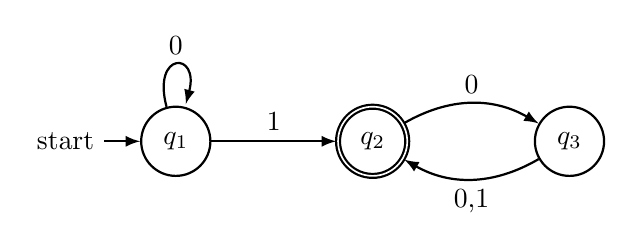
\begin{tikzpicture}[->,>=latex,thick,auto,node distance=2.5cm]
    \node[state,initial] (q1) {$q_1$};
    \node[state,accepting] (q2) [right of=q1] {$q_2$};
    \node[state] (q3) [right of=q2] {$q_3$};
    \path (q1) edge [loop above] node {0} (q1)
          (q1) edge node {1} (q2)
          (q2) edge [bend left] node {0} (q3)
          (q3) edge [bend left] node {0,1} (q2);
  \end{tikzpicture}
\end{Verbatim}
  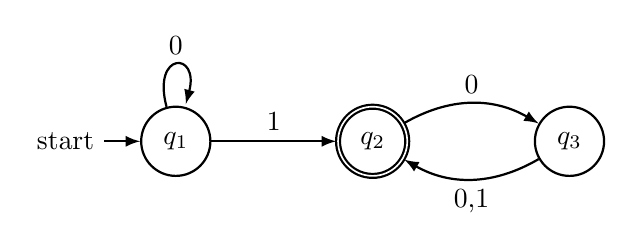
\begin{tikzpicture}[->,>=latex,thick,auto,node distance=2.5cm]
    \node[state,initial] (q1) {$q_1$};
    \node[state,accepting] (q2) [right of=q1] {$q_2$};
    \node[state] (q3) [right of=q2] {$q_3$};
    \path (q1) edge [loop above] node {0} (q1)
          (q1) edge node {1} (q2)
          (q2) edge [bend left] node {0} (q3)
          (q3) edge [bend left] node {0,1} (q2);
  \end{tikzpicture}

  \newpage
  
\begin{Verbatim}[frame=single]  
  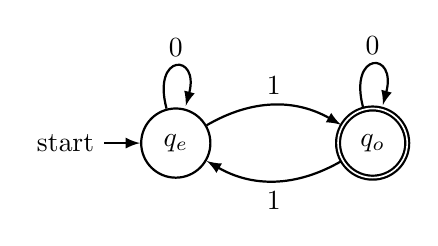
\begin{tikzpicture}[->,>=latex,thick,auto,node distance=2.5cm]
    \node[state,initial] (e) {$q_e$};
    \node[state,accepting] (o) [right of=e] {$q_o$};
    \path (e) edge [loop above] node {0} (e)
          (e) edge [bend left] node {1} (o)
          (o) edge [bend left] node {1} (e)
          (o) edge [loop above] node {0} (e);
  \end{tikzpicture}
\end{Verbatim}
  
  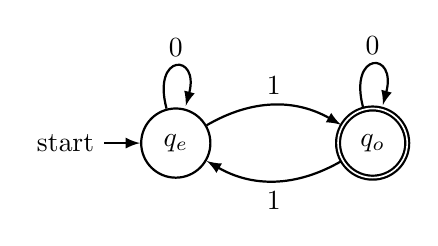
\begin{tikzpicture}[->,>=latex,thick,auto,node distance=2.5cm]
    \node[state,initial] (e) {$q_e$};
    \node[state,accepting] (o) [right of=e] {$q_o$};
    \path (e) edge [loop above] node {0} (e)
          (e) edge [bend left] node {1} (o)
          (o) edge [bend left] node {1} (e)
          (o) edge [loop above] node {0} (e);
  \end{tikzpicture}
  \begin{Verbatim}[frame=single]
  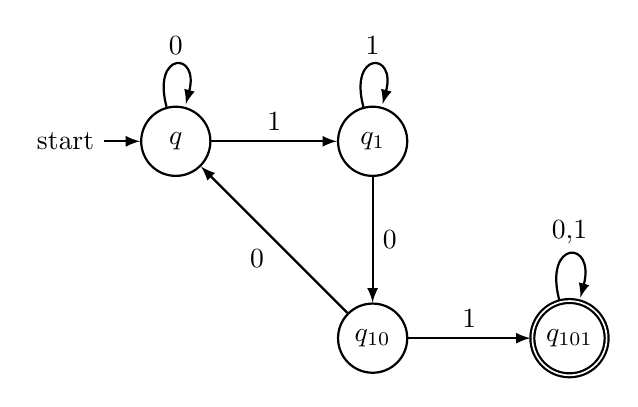
\begin{tikzpicture}[->,>=latex,thick,auto,node distance=2.5cm]
    \node[state,initial] (q) {$q$};
    \node[state] (1) [right of=q] {$q_1$};
    \node[state] (10) [below of=1] {$q_{10}$};
    \node[state,accepting] (101) [right of=10] {$q_{101}$};
    \path (q) edge [loop above] node {0} (q)
          (q) edge node {1} (1)
          (1) edge [loop above] node {1} (1)
          (1) edge node {0} (10)
          (10) edge node {0} (q)
          (10) edge node {1} (101)
          (101) edge [loop above] node {0,1} (101);
  \end{tikzpicture}
\end{Verbatim}
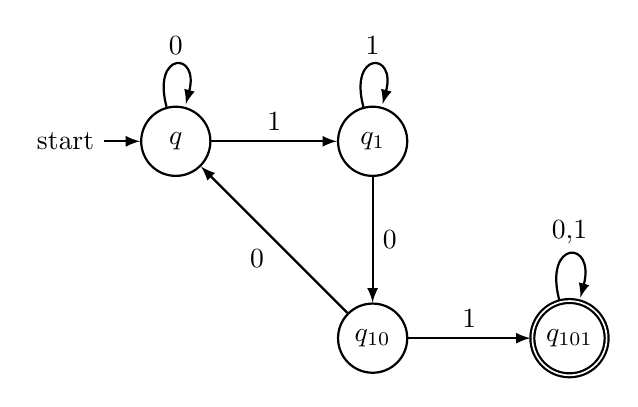
\begin{tikzpicture}[->,>=latex,thick,auto,node distance=2.5cm]
  \node[state,initial] (q) {$q$};
  \node[state] (1) [right of=q] {$q_1$};
  \node[state] (10) [below of=1] {$q_{10}$};
  \node[state,accepting] (101) [right of=10] {$q_{101}$};
  \path (q) edge [loop above] node {0} (q)
  (q) edge node {1} (1)
  (1) edge [loop above] node {1} (1)
  (1) edge node {0} (10)
  (10) edge node {0} (q)
  (10) edge node {1} (101)
  (101) edge [loop above] node {0,1} (101);
\end{tikzpicture}

\newpage
\begin{Verbatim}[frame=single]
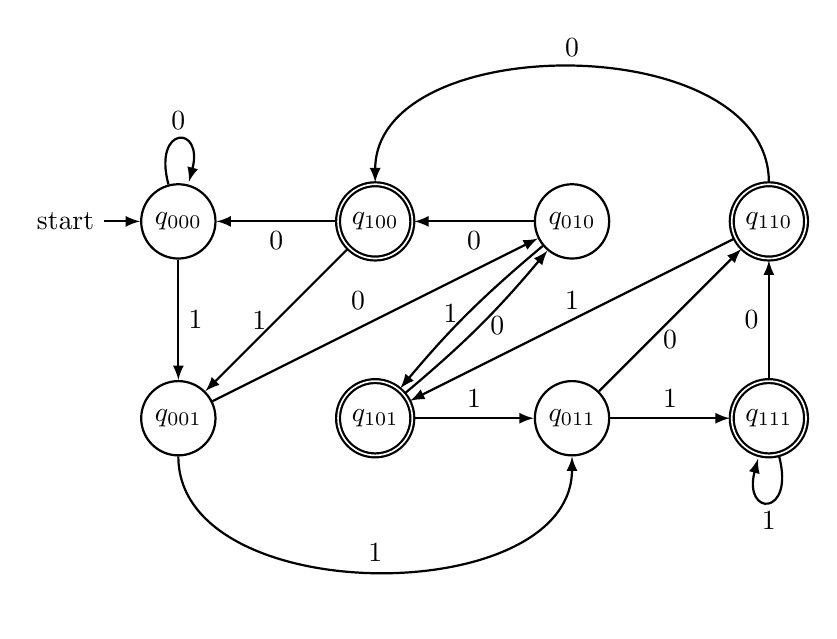
\begin{tikzpicture}[->,>=latex,thick,auto,node distance=2.5cm]
  \node[state,initial] (000) {$q_{000}$};
  \node[state,accepting] (100) [right of=000] {$q_{100}$};
  \node[state] (010) [right of=100] {$q_{010}$};
  \node[state,accepting] (110) [right of=010] {$q_{110}$};
  \node[state] (001) [below of=000] {$q_{001}$};
  \node[state,accepting] (101) [right of=001] {$q_{101}$};
  \node[state] (011) [right of=101] {$q_{011}$};
  \node[state,accepting] (111) [right of=011] {$q_{111}$};
  \path (000) edge [loop above] node {0} (000)
  (000) edge node {1} (001)
  (100) edge node {0} (000)
  (100) edge node [left] {1} (001)
  (010) edge node {0} (100)
  (010) edge [out=-140,in=50] node [left] {1} (101)
  (110) edge [out=90, in=90] node [above] {0} (100)
  (110) edge node [above] {1} (101)
  (001) edge node {0} (010)
  (001) edge [out=-90, in=-90] node {1} (011)
  (101) edge [out=40,in=-130] node [right] {0} (010)
  (101) edge node {1} (011)
  (011) edge node [below] {0} (110)
  (011) edge node {1} (111)
  (111) edge node {0} (110)
  (111) edge [loop below] node {1} (111);
\end{tikzpicture}
\end{Verbatim}
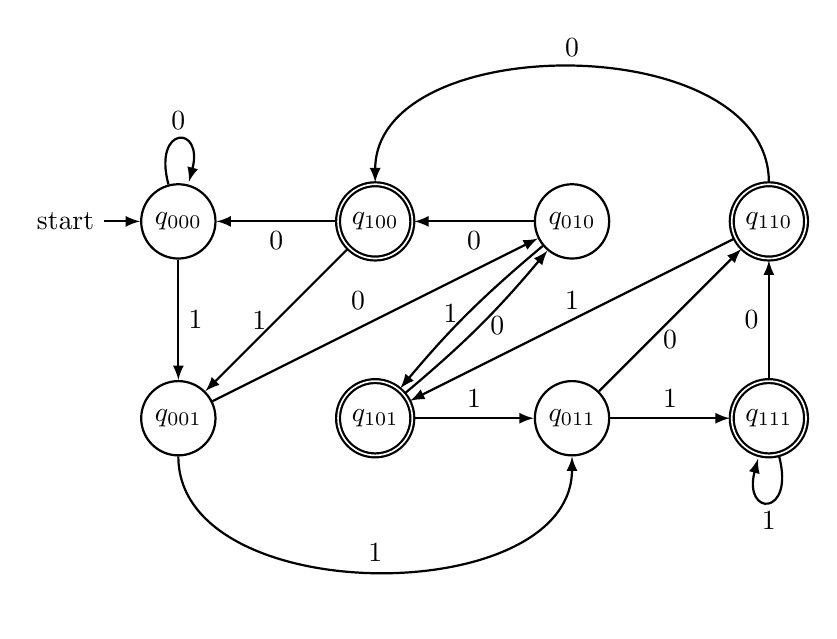
\begin{tikzpicture}[->,>=latex,thick,auto,node distance=2.5cm]
  \node[state,initial] (000) {$q_{000}$};
  \node[state,accepting] (100) [right of=000] {$q_{100}$};
  \node[state] (010) [right of=100] {$q_{010}$};
  \node[state,accepting] (110) [right of=010] {$q_{110}$};
  \node[state] (001) [below of=000] {$q_{001}$};
  \node[state,accepting] (101) [right of=001] {$q_{101}$};
  \node[state] (011) [right of=101] {$q_{011}$};
  \node[state,accepting] (111) [right of=011] {$q_{111}$};
  \path (000) edge [loop above] node {0} (000)
  (000) edge node {1} (001)
  (100) edge node {0} (000)
  (100) edge node [left] {1} (001)
  (010) edge node {0} (100)
  (010) edge [out=-140,in=50] node [left] {1} (101)
  (110) edge [out=90, in=90] node [above] {0} (100)
  (110) edge node [above] {1} (101)
  (001) edge node {0} (010)
  (001) edge [out=-90, in=-90] node {1} (011)
  (101) edge [out=40,in=-130] node [right] {0} (010)
  (101) edge node {1} (011)
  (011) edge node [below] {0} (110)
  (011) edge node {1} (111)
  (111) edge node {0} (110)
  (111) edge [loop below] node {1} (111);
\end{tikzpicture}

\newpage
The same thing with a matrix:

\begin{Verbatim}[frame=single]
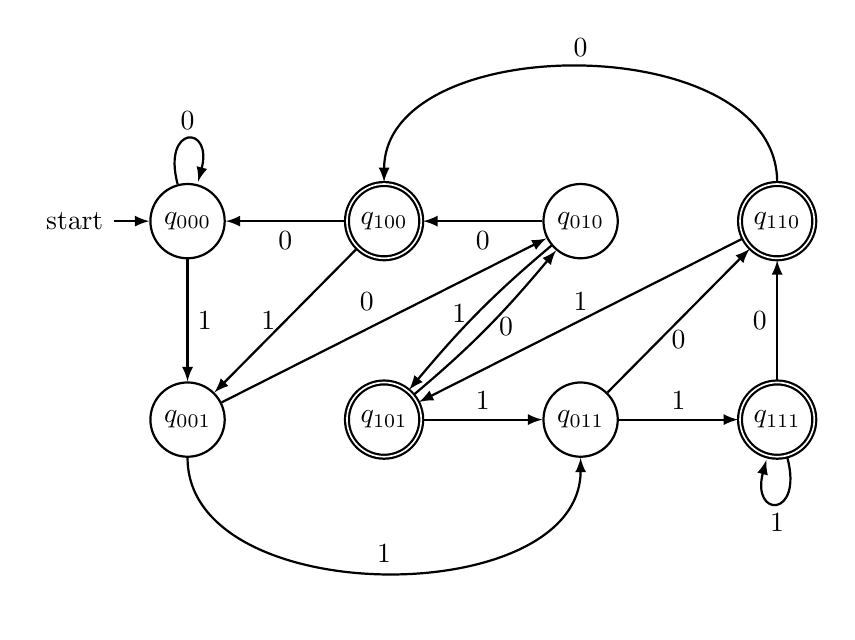
\begin{tikzpicture}[->,>=latex,thick,auto]
  \matrix[row sep=1.5cm,column sep=1.5cm]{
    \node[state,initial] (000) {$q_{000}$}; &
    \node[state,accepting] (100)  {$q_{100}$}; &
    \node[state] (010) {$q_{010}$}; &
    \node[state,accepting] (110)  {$q_{110}$};\\
    \node[state] (001) {$q_{001}$}; &
    \node[state,accepting] (101)  {$q_{101}$}; &
    \node[state] (011) {$q_{011}$}; &
    \node[state,accepting] (111)  {$q_{111}$};\\
  };
  \path (000) edge [loop above] node {0} (000)
  (000) edge node {1} (001)
  (100) edge node {0} (000)
  (100) edge node [left] {1} (001)
  (010) edge node {0} (100)
  (010) edge [out=-140,in=50] node [left] {1} (101)
  (110) edge [out=90, in=90] node [above] {0} (100)
  (110) edge node [above] {1} (101)
  (001) edge node {0} (010)
  (001) edge [out=-90, in=-90] node {1} (011)
  (101) edge [out=40,in=-130] node [right] {0} (010)
  (101) edge node {1} (011)
  (011) edge node [below] {0} (110)
  (011) edge node {1} (111)
  (111) edge node {0} (110)
  (111) edge [loop below] node {1} (111);
\end{tikzpicture}
\end{Verbatim}
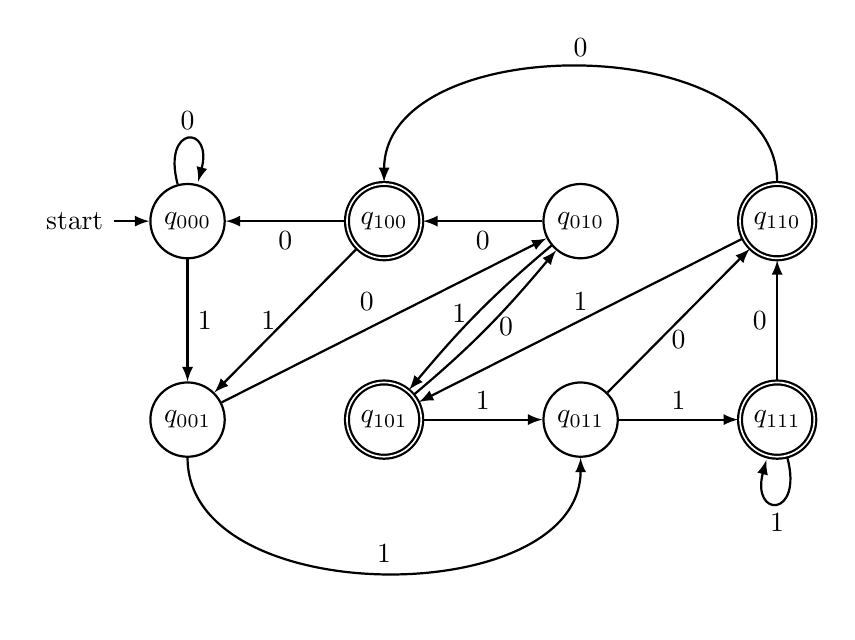
\begin{tikzpicture}[->,>=latex,thick,auto]
  \matrix[row sep=1.5cm,column sep=1.5cm]{
    \node[state,initial] (000) {$q_{000}$}; &
    \node[state,accepting] (100)  {$q_{100}$}; &
    \node[state] (010) {$q_{010}$}; &
    \node[state,accepting] (110)  {$q_{110}$};\\
    \node[state] (001) {$q_{001}$}; &
    \node[state,accepting] (101)  {$q_{101}$}; &
    \node[state] (011) {$q_{011}$}; &
    \node[state,accepting] (111)  {$q_{111}$};\\
  };
  \path (000) edge [loop above] node {0} (000)
  (000) edge node {1} (001)
  (100) edge node {0} (000)
  (100) edge node [left] {1} (001)
  (010) edge node {0} (100)
  (010) edge [out=-140,in=50] node [left] {1} (101)
  (110) edge [out=90, in=90] node [above] {0} (100)
  (110) edge node [above] {1} (101)
  (001) edge node {0} (010)
  (001) edge [out=-90, in=-90] node {1} (011)
  (101) edge [out=40,in=-130] node [right] {0} (010)
  (101) edge node {1} (011)
  (011) edge node [below] {0} (110)
  (011) edge node {1} (111)
  (111) edge node {0} (110)
  (111) edge [loop below] node {1} (111);
\end{tikzpicture}




\end{document}
